\documentclass[12pt,a4paper]{book}
\usepackage[left=2.00cm, right=2.00cm, top=2.00cm, bottom=2.00cm]{geometry}
\usepackage[utf8]{inputenc}
\usepackage[ngerman]{babel}
\usepackage{graphicx}
\usepackage{subcaption} 
\begin{document}
Abbildung \ref{fig:subhouses} besteht aus Abbildung \ref{fig:subhouse1} und Abbildung \ref{fig:subhouse2}.
\begin{figure}[htb]
	\centering
	\subcaptionbox{Erstes Haus\label{fig:subhouse1}}
	{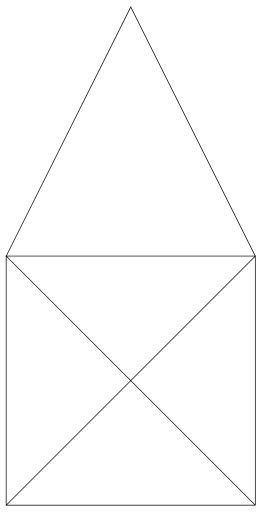
\includegraphics[width=3cm]{house/house.png}}
	\hfil
	\subcaptionbox{Zweites Haus\label{fig:subhouse2}}
	{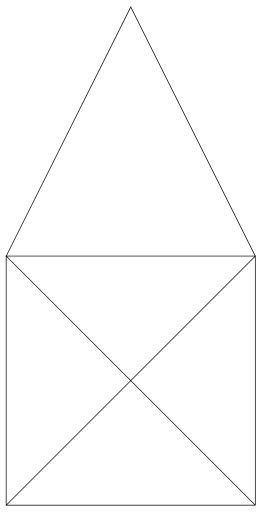
\includegraphics[width=3cm,angle=180]{house/house.png}}
	\caption{Zwei Häuser}\label{fig:subhouses}
\end{figure}

Abbildung \ref{fig:subhouses2} besteht aus Abbildung \ref{fig:subhouse21} und Abbildung \ref{fig:subhouse22}.
\begin{figure}[hbt]
	\begin{subfigure}[b]{.5\linewidth} 
		\centering
		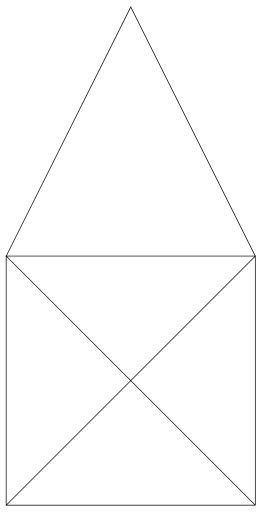
\includegraphics[width=3cm]{house/house.png}
		\caption{Erstes Haus}\label{fig:subhouse21}
	\end{subfigure}
	\hfil
	\begin{subfigure}[b]{.5\linewidth}
		\centering
		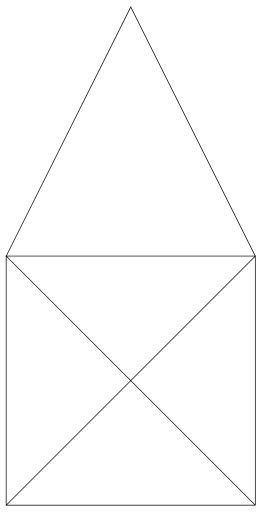
\includegraphics[width=3cm,angle=180]{house/house.png}
		\caption{Zweites Haus}\label{fig:subhouse22}
	\end{subfigure}
	\caption{Zwei Häuser}\label{fig:subhouses2}
\end{figure}
\end{document}